% ========================================
% CHAPTER 5: EXPERIMENTS AND EVALUATION (ACTUAL SETUPS AND RESULTS)
% ========================================
\chapter{Experiments and Evaluation}

% ========================================
% SECTION 5.0: EXPERIMENTAL SETUP
% ========================================
\section{Experimental Setup}

We implement our ICAE framework from scratch, building upon the original architecture \cite{ge_-context_2024} with several modifications for improved efficiency and reproducibility. Our implementation uses Qwen3-8B as the base model, with LoRA adaptation applied to the attention matrices (q\_proj and v\_proj) using a rank of 128.

Pretraining is conducted on the SlimPajama-6B dataset using a combination of autoencoding and language modeling objectives, achieving 95\% reconstruction BLEU score on general text. Fine-tuning on SWE-bench trajectories uses a larger memory size of 256 tokens and explicitly disables thinking mechanisms for simplicity, focusing on direct tool-call generation.

Training was performed on a single NVIDIA H200 GPU, requiring approximately 1 day and 15 hours for pretraining and 3 days for fine-tuning due to the computational complexity of the autoencoding objective and resulting lack of effective batching opportunities.

Detailed hyperparameters and training configurations are provided in Appendix~\ref{app:training_details}.


% ========================================
% SECTION 5.1: INITIAL PROTOTYPE EXPERIMENTS: THE NECESSITY OF TRAINING
% ========================================
\section{Initial Prototype Experiments: The Necessity of Training}

The initial approach tested replacing hard tokens with soft/averaged continuous embeddings without fine-tuning.
These prototype experiments, using methods like KV-cache hacks or direct embedding inputs in vLLM, demonstrated that scores decreased by more than 50\% on QA tasks (e.g., SQuAD context embed F1 dropped from 0.71 to 0.17 or 0.11).
This negative result confirmed the hypothesis that training is necessary to effectively condense context into the latent space.

\begin{table}[h]
    \centering
    \begin{tabular}{lcc}
        \toprule
        \textbf{Setting (SQuAD), context embed} &
        \textbf{Exact Match} & \textbf{F1} \\
        \midrule
        Baseline — hard tokens         & \textbf{0.58} & \textbf{0.71} \\
        Hard embedded, avg ×2          & 0.09 & 0.21 \\
        Soft embedded online, avg ×2          & 0.05 & 0.11 \\
        Soft embedded \text{regenerate-llm} avg ×2          & 0.07 & 0.16 \\
        \bottomrule
    \end{tabular}
    \caption{Baseline against averaging techniques (Prompt–Q–C)}
    \label{tab:avg_variants}
\end{table}

\begin{figure}[hbt]
  \centering
  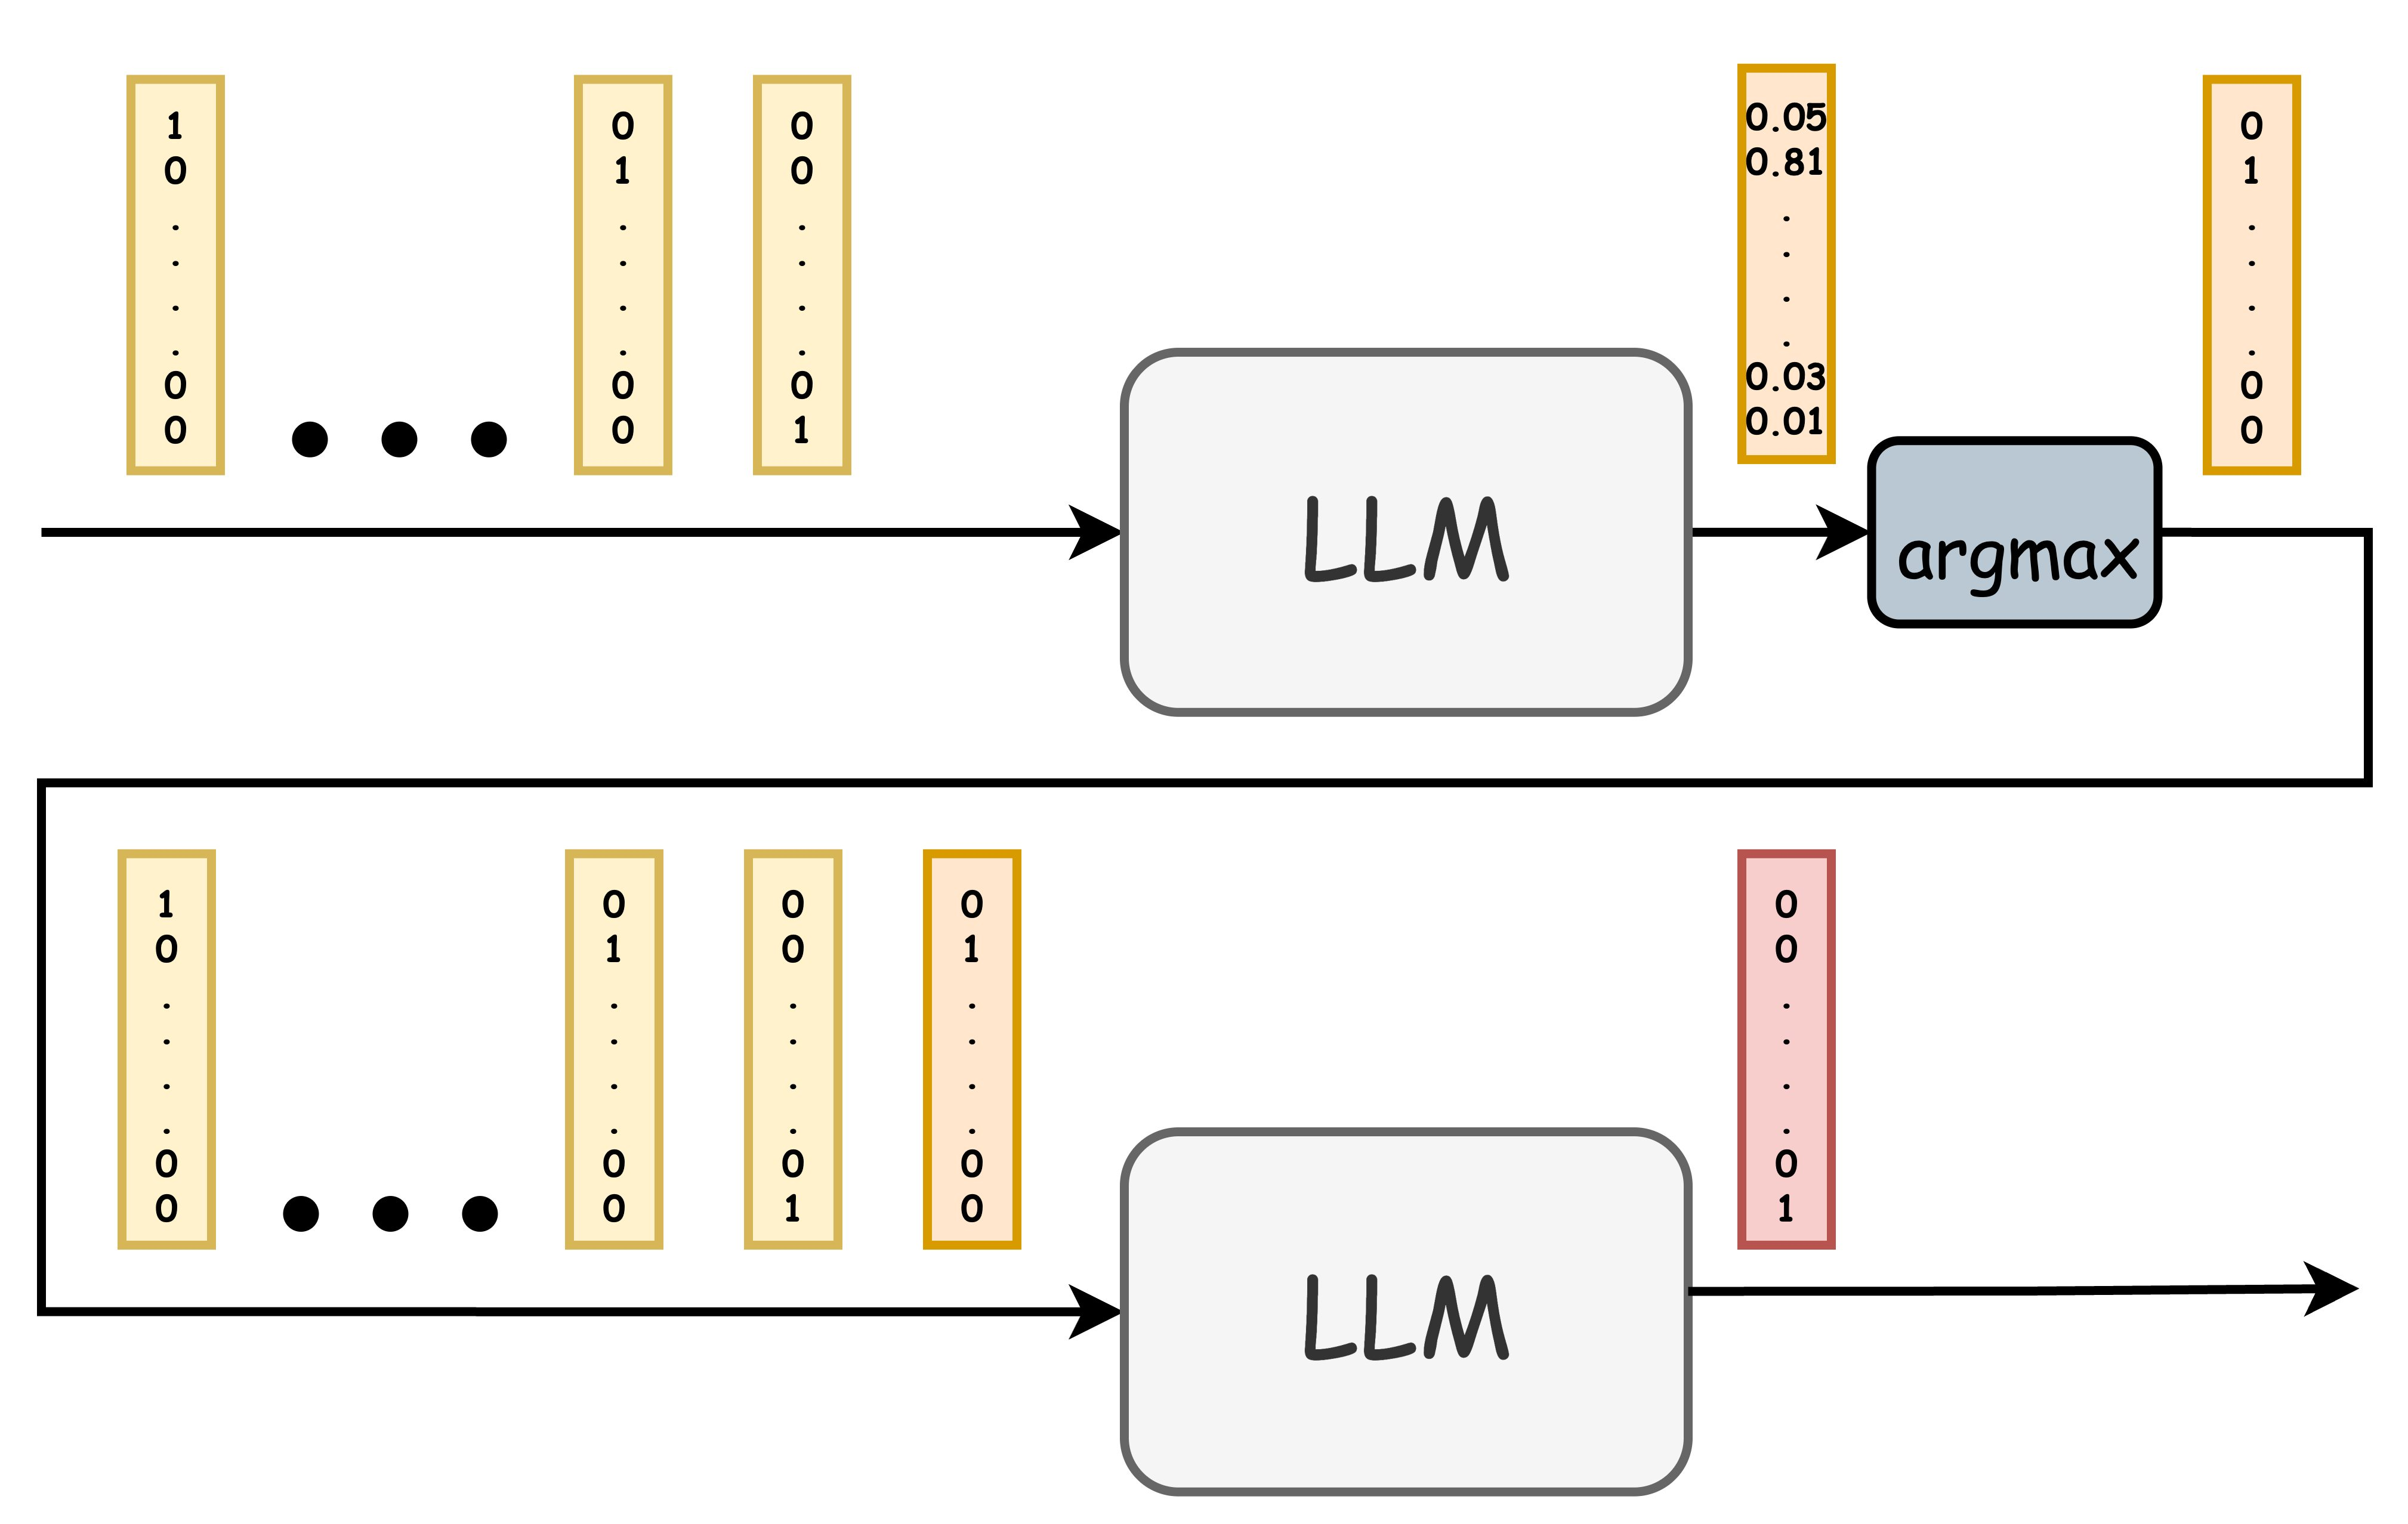
\includegraphics[width=0.8\textwidth]{graphs/ser1.jpeg}
  \caption{Results of the "without training" approach - SER1}
  \label{fig:ser1}
\end{figure}

\begin{figure}[hbt]
  \centering
  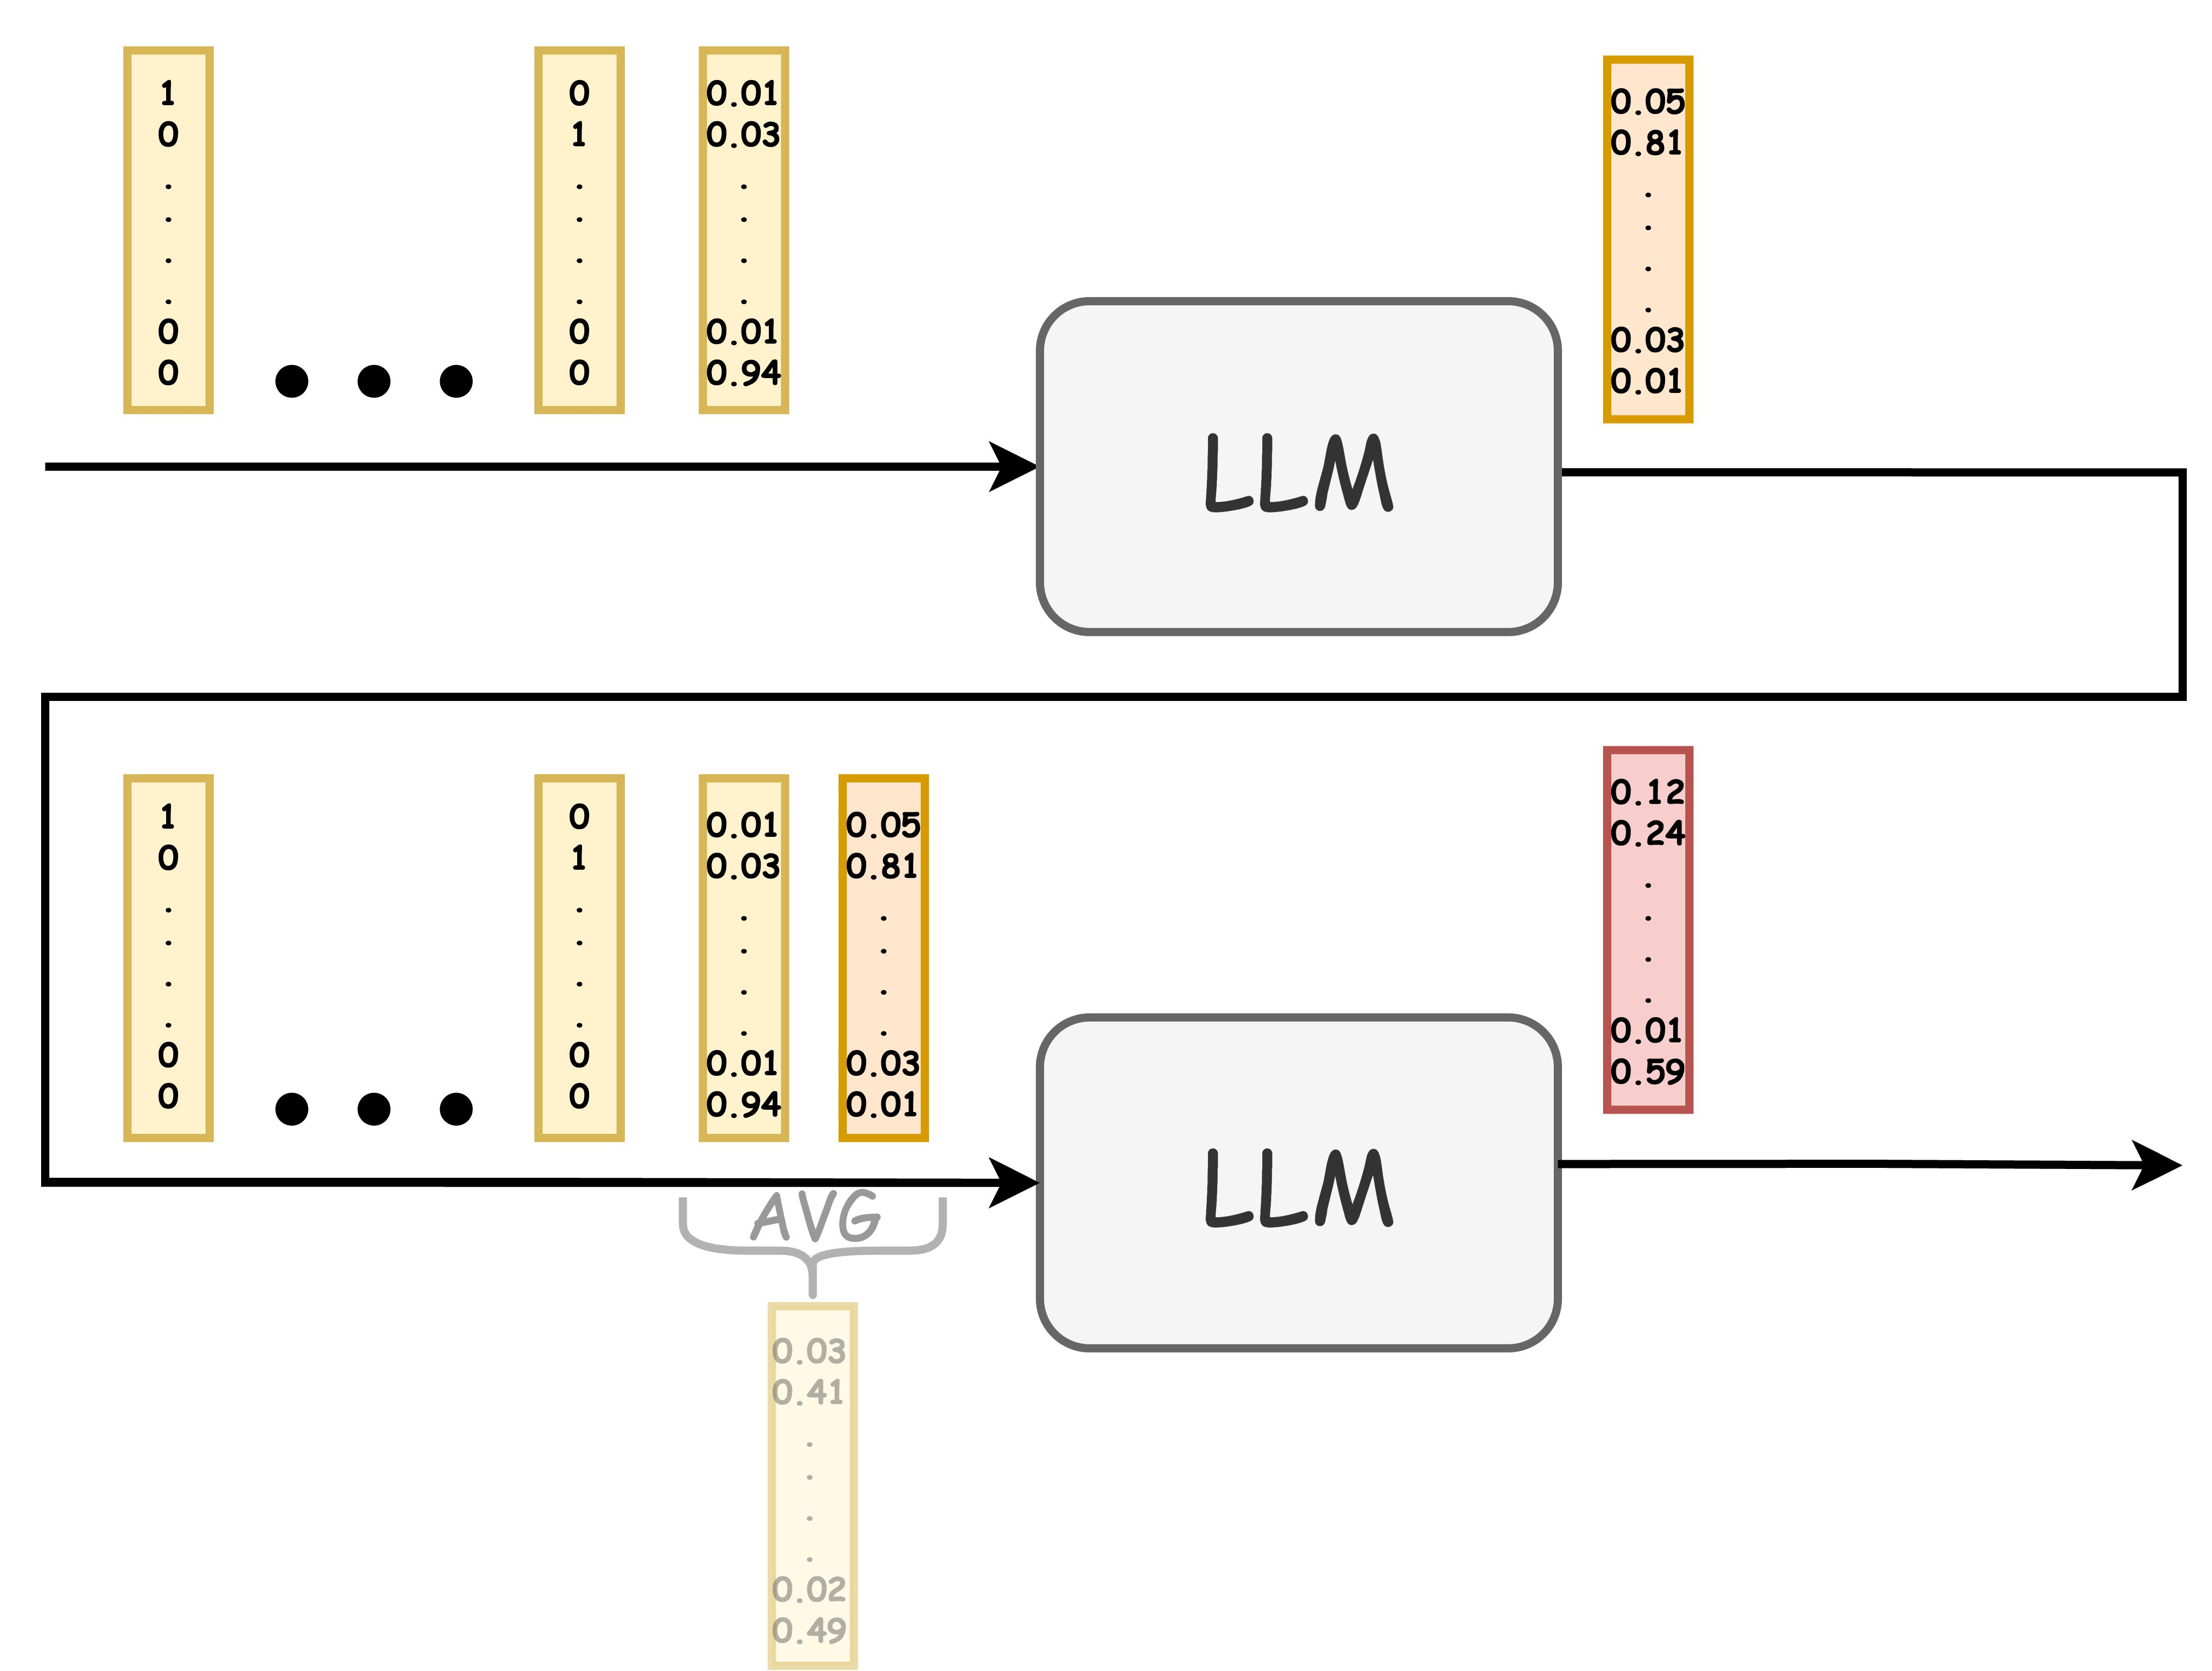
\includegraphics[width=0.8\textwidth]{graphs/ser2.jpeg}
  \caption{Results of the "without training" approach - SER2}
  \label{fig:ser2}
\end{figure}


% ========================================
% SECTION 5.2: EVALUATION ON GENERAL TEXT RECONSTRUCTION
% ========================================
\section{Evaluation on General Text Reconstruction}

Pretrained ICAE \cite{ge_-context_2024} demonstrated the ability to decompress general texts almost perfectly.
High BLEU scores were achieved on datasets like PWC (99.1 for Mistral-7B, 99.5 for Llama-2-7B) and SQuAD (98.1 for Qwen3-8B), indicating that memory slots retained almost all context information for contexts up to 400 tokens.
Analysis of reconstruction errors showed patterns similar to human memorization mistakes (e.g., restoring "large pretrained language model" as "large pretrained model"), suggesting the model selectively emphasizes or neglects information based on its understanding.


% ========================================
% SECTION 5.3: EVALUATION ON QUESTION ANSWERING TASKS (OFFLINE)
% ========================================
\section{Evaluation on Question Answering Tasks (Offline)}

When fine-tuned on QA tasks (SQuAD), ICAE-FT \cite{ge_-context_2024} achieved high F1 (73) and Exact Match (69\%) scores, performing well compared to LoRA-FT baselines.
The quality of the compressed representation was shown to significantly outperform summaries generated by GPT-4 under the same length constraint (128 tokens).

\begin{table}[h]
    \centering
    \begin{tabular}{lccc}
        \toprule
        \textbf{Model} &
        \textbf{Compression} &
        \textbf{Exact Match} &
        \textbf{F1} \\
        \midrule
        Mistral-7B (no FT)          & ×$1$         & 49 & 68 \\
        LoRA-FT baseline            & ×$1$         & \underline{59} & \underline{65} \\
        ICAE FT (PwC, authors)       & ×$1.7\pm0.7$ & 41 & 57 \\
        ICAE FT (SQuAD, ours)              & ×$1.7\pm0.7$ & \textbf{69} & \textbf{73} \\
        \bottomrule
    \end{tabular}
    \caption{ICAE averaging on SQuAD}
    \label{tab:icae_squad}
\end{table}


% ========================================
% SECTION 5.4: EVALUATION ON AGENTIC PERFORMANCE (SWE-BENCH)
% ========================================
\section{Evaluation on Agentic Performance (SWE-bench)}

Efficiency Results: ICAE \cite{ge_-context_2024} compression led to measurable efficiency improvements, achieving a theoretically 10\% faster mean tool-call generation time than the vanilla baseline (e.g., 0.4880s vs 0.5437s).
Furthermore, latency tests showed speedups of 2.2× to 3.6× in total time for inference.
Token-wise Accuracy vs. Resolved Rate: Although token-wise accuracy performed on par with (or slightly better than) the vanilla Qwen baseline (e.g., 0.9089 vs 0.9000), this metric was noted to be problematic ("token-wise accuracy is bullshit") and decoupled from true task success.
End-to-End Task Success: The primary negative finding was that the model with compression resolved significantly fewer than 50\% as many issues as the original Qwen model on the SWE-bench Verified dataset.

\begin{table}[h]
    \centering
    \setlength{\tabcolsep}{6pt}
    \begin{tabular}{llcc}
        \toprule
        \textbf{Encoder} & \textbf{Decoder} & \textbf{Accuracy} & \textbf{Mean tool-call time (s)} \\
        \midrule
        % --- Baseline encoder
        —                        & Full-FT   & 0.9484 & 1.24 \\
        —                        & LoRA-FT   & 0.9118 & 1.24 \\
        —                        & Qwen           & 0.8967 & 1.23 \\
        \addlinespace
        % --- Ablations
        del long obs-s             & Qwen           & 0.8873 & 0.44 \\
        del all obs-s              & Qwen           & 0.8802 & 0.39 \\
        \addlinespace
        % --- ICAE (Qwen pretrained) encoder
        ICAE (LoRA-PT w/ Full-FT)   & Full-FT   &  0.9219    &  — \\
        ICAE (LoRA-PT w/ Qwen)    & Qwen           &  0.8808 & \textbf{1.12 (0.31+0.81)} \\
        \addlinespace
        % --- ICAE (Qwen-LoRA-FT) encoder
        ICAE (LoRA-FT)         & Full-FT   &  ?   & —  \\
        ICAE (LoRA-FT)         & LoRA-FT   & 0.9263   & —  \\
        ICAE (LoRA-FT)         & Qwen           & 0.9020 & — \\
        % bad-seed ICAE (LoRA-FT)         & Qwen           & 0.8918 & — \\       

        
        \bottomrule
    \end{tabular}
    \caption{No think bug table. Qwen and ICAE future variants. FT=FineTuning, PT=PreTraining}
    \label{tab:icae_variants}
\end{table}

\begin{table}[h]
    \centering
    \small
    \setlength{\tabcolsep}{4pt}
    % --- Добавлены рамки по краям таблицы для цельного вида ---
    \begin{tabular}{|ll|ccc|}
        \hline
        \textbf{Encoder} & \textbf{Decoder} & \textbf{Acc.} & \textbf{Time (s)} & \textbf{Resolved (/500)} \\
        \hline
        % --- Baseline encoder
        —                         & Qwen-Full-FT   & 0.9484 & 1.24                      & —         \\
        —                         & Qwen-LoRA-FT   & 0.9118 & 1.24                      & 10        \\
        —                         & Qwen           & 0.8967 & 1.23                      & 26        \\
        \hline
        % --- ICAE (Qwen-LoRA-FT) encoder
        ICAE (Qwen-LoRA-FT)       & Qwen           & 0.9020 & —                         & 11        \\
        ICAE (Qwen-LoRA-FT)       & Qwen-LoRA-FT   & 0.9263 & —                         & 3 (overfit?) \\
        ICAE (Qwen-LoRA-FT)       & Qwen-Full-FT   & ?      & —                         & —         \\
        \hline
        % --- Ablations
        del long obs-s            & Qwen           & 0.8873 & 0.44                      & 1         \\
        del all obs-s             & Qwen           & 0.8802 & 0.39                      & 0         \\
        \hline
        % --- ICAE (Qwen pretrained) encoder
        ICAE (Qwen-LoRA-PT w/ Q-Full-FT) & Qwen-Full-FT   & 0.9219 & —                         & —         \\
        ICAE (Qwen-LoRA-PT w/ Qwen)      & Qwen           & 0.8808 & \textbf{1.12 (0.31+0.81)} & —         \\
        \hline
    \end{tabular}
    \caption{No think bug table. Qwen and ICAE future variants. FT=FineTuning, PT=PreTraining}
    \label{tab:qwen_icae_variants_absolute}
\end{table}

\begin{figure}[hbt]
  \centering
  
\includegraphics[width=0.8\textwidth]{graphs/mega-1.jpeg}
  \caption{ICAE application to SWE-bench - Results 1}
  \label{fig:mega1}
\end{figure}

\begin{figure}[hbt]
  \centering
  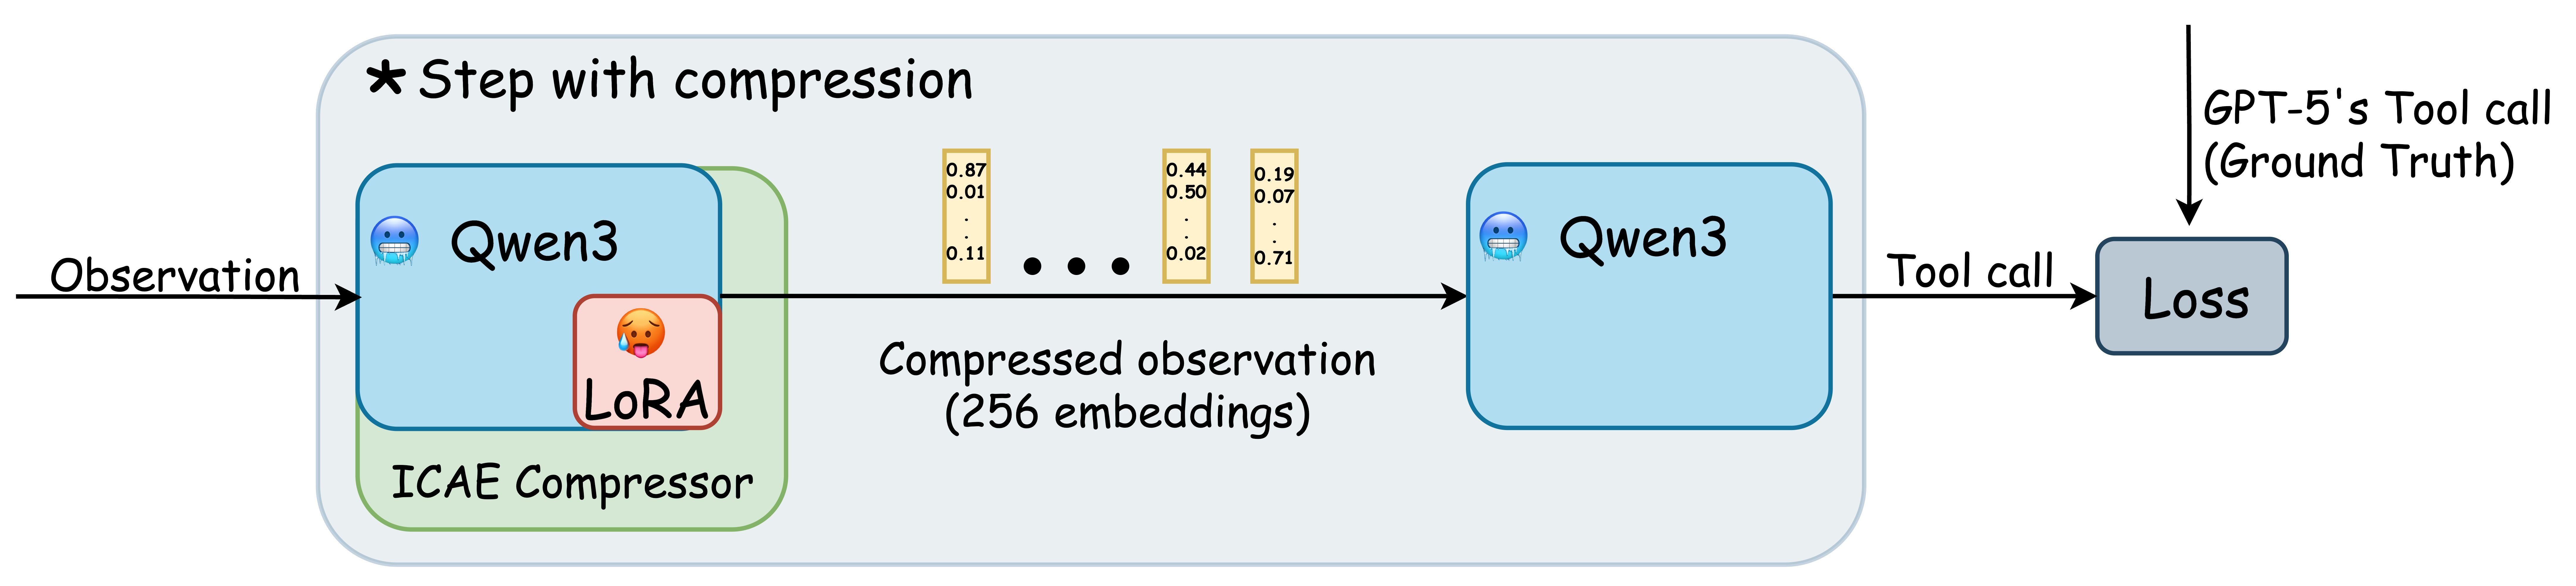
\includegraphics[width=0.8\textwidth]{graphs/mega-2.jpeg}
  \caption{ICAE application to SWE-bench - Results 2}
  \label{fig:mega2}
\end{figure}


% ========================================
% SECTION 5.5: DISCUSSION OF AGENTIC FAILURE HYPOTHESES
% ========================================
\section{Discussion of Agentic Failure Hypotheses}

Hypotheses for the end-to-end performance degradation include Representation–behavior mismatch, where the compression perturbs the decoder's behavior necessary for tool use.
Other factors include reconstruction quality falloff for specialized content like code files, and potential overfitting to labels demonstrated by high local accuracy but low resolved rates.
